\section*{Prefácio}

Este texto tem como propósito primordial (1) atender à necessidade de um material que apresente os tópicos abordados na disciplina de \textit{Estrutura de Dados} de forma organizada e (2) oferecer suporte a estudantes que não tenham cursado a disciplina de \textit{Matemática Discreta}, promovendo um encontro mais suave com os tópicos em matemática do conteúdo.

O texto está sendo aprimorado, e ficarei grato por qualquer sugestão ou comentário que você (leitor) possa enviar para o e-mail: \href{mailto:augustoguerradelima@proton.me}{augustoguerradelima@proton.me}.
\vspace{0.5cm}

{\raggedleft
Belo Horizonte, fevereiro de 2024

Augusto Guerra de Lima
\par}

\newpage
\section{Complexidade de algoritmos}
\

Antes de tudo, uma pergunta simples: Quantas comparações o laço de iteração abaixo deve fazer até parar?

\begin{lstlisting}[language=C, frame=single]
    for(i:=0; i<n; i++)
\end{lstlisting}

O laço realiza $n+1$ comparações e repete $n$ vezes. Esse tipo de contagem é importante para determinar a complexidade de um algoritmo, isso será feito junto de uma notação matemática chamada \textbf{notação assintótica}.

Tempo de execução, armazenamento e robustez são algumas características que determinam a qualidade de um algoritmo.

A \textbf{complexidade do tempo de execução} de um algoritmo é avaliada para estimar sua eficiência antes da implementação. A eficiência é representada por uma função que recebe o tamanho da entrada do algoritmo como parâmetro.

\subsection{Crescimento assintótico de funções}
\

A \textbf{análise assintótica} avalia o comportamento de uma função para valores de parâmetros \textit{significativamente grandes}. Por exemplo, ao ver a expressão $n^2+10$ é comum pensar em valores pequenos de $n$, a análise assintótica se preocupa com valores enormes de $n$ onde a constante $10$ por exemplo, não faria diferença e o termo $n^2$ dominaria assintoticamente o crescimento da função.

As notações utilizadas para descrever complexidade são definidas em termos de funções cujos domínios são o conjunto dos números inteiros não negativos. Definiremos que $\mathbb{N}_0 = \{0,1,2...\}$ e $\mathbb{R}^{+}$ como o conjunto dos números reais não negativos.

Sejam $f$ e $g$ funções tais que a taxa de crescimento de $f$ é maior que a de $g$, podemos denotar $g\prec f$.

Antes de introduzir a notação assintótica, vamos avaliar um exemplo preliminar.

\textbf{Exemplo 1 (Comparando funções)}

Sejam $f$ e $g$ funções definidas no conjunto dos números inteiros não negativos, para comparar o comportamento assintótico de $g$ e $f$, é preciso encontrar uma constante $k$ tal que $g(n)\leq kf(n)$ para todo $n$ suficientemente grande (escreveremos $n\geq n_0$). Isto é, encontrar constantes $k$ e $n_0$.

Sabendo $g(n)=\lceil\frac{n}{2}\rceil+10$ e $f(n)=n$, encontrar $k$ e $n_0$ tais que $g(n)\leq kf(n), \forall n\geq n_0$.

\[\Bigr\lceil \frac{n}{2} \Bigr\rceil \leq kn; \ \ \ \Bigr\lceil \frac{n}{2} \Bigr\rceil \leq \frac{n}{2} + 11 \leq \frac{n}{2} + \frac{n}{2} = n.\]

Se $k=1$ e $n_0=21$, por exemplo, então $f(n_0)=\lceil\frac{21}{2}\rceil+10 = 21$ e $g(n_0)=21$ e uma solução foi encontrada. Podem haver mais soluções.

{\raggedleft $\bigtriangleup$ \par}

\textbf{Exemplo 2 (Caso sem solução)}

Se $g(n)=n^3$ e $f(n)=n^2$, encontrar $k$ e $n_0$ tais que $g(n)\leq kf(n), \ \forall n\geq n_0$.
\[n^3\leq kn^2 \Rightarrow n\leq k, \ \forall n\geq n_0. \]
É impossível que uma função linear seja sempre menor ou igual a uma constante, portanto não há solução.

{\raggedleft $\bigtriangleup$ \par}

\subsubsection{Notação $O$}
\

A notação $O(f(n))$ (O grande de $f$ de $n$), é o \textbf{limite assintótico superior justo} é a mais utilizada para descrever a complexidade de um algoritmo. Para uma função $f(n)$, $O(f(n))$ é o conjunto de funções

\[O(f(n)) = \{g: \mathbb{N}_0 \rightarrow \mathbb{R}^{+}: \ \exists k, \ n_0 > 0 ; \ 0\leq g(n) \leq kf(n), \ \forall n \geq n_0\}.\]
$O(f(n))=$ \{"Todas as funções que têm taxa de crescimento menor ou igual a $f(n)$"\}.

Dizer $g(n) \in O(f(n))$ é dar um limite superior para $g(n)$, ou seja, intuitivamente para todos os valores $n\geq n_0$, encontrar uma família de funções com taxa de crescimento maior que $g(n)$. A figura 1 mostra um exemplo gráfico.

Utilizando a notação $O$, muitas vezes é possível determinar o tempo de execução de um algoritmo apenas inspecionando sua estrutura global. Um laço de iteração que fizer $n + 1$ comparações por exemplo, tem tempo de execução $O(n)$.

\textbf{Exemplo}

Sejam $g(n)=2n^2 + n$ e $f(n)=n^2$, é verdadeiro que $g(n)\in O(f(n))$ ou melhor, $2n^2 + n \in O(n^2)$.

Substituindo na desigualdade e simplificando os termos
\[2n^2+n\leq kn^2 \Rightarrow 2 + \frac{1}{n}\leq k \forall n\geq n_0\]

$k=3$ e $n_0=1$ satisfazem $g(n)\in O(f(n))$. Basta substituir os valores na desigualdade e verificar

\[2n^2+n\leq 3n^2 \Rightarrow n\leq n^2\]

A desigualdade é verdadeira para todo $n\geq 1$, em outras palavras $n_0=1$.

{\raggedleft $\bigtriangleup$ \par}

\begin{figure}
  \centering
  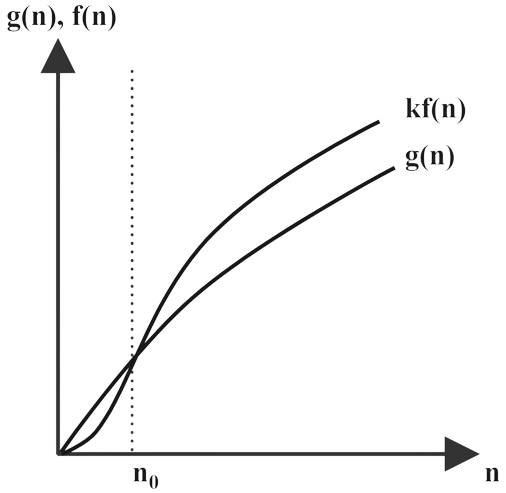
\includegraphics[width=0.4\linewidth]{img/O(f(n)).png}
    \caption{$g(n)\in O(f(n))$.}
    \label{O(f(n))}
\end{figure}

\subsubsection{Notação $\Omega$}
\

A notação $\Omega(f(n))$ (Ômega de $f$ de $n$), é o \textbf{limite assintótico inferior justo}. Nesse caso, dizer $g(n)=\Omega(f(n))$, significa que existe uma constante $k$ tal que $0 \leq kf(n) \leq g(n)$ para todo $n \geq n_0$. Para uma função $f(n)$, $\Omega(f(n))$ é o conjunto de funções

\[\Omega(f(n)) = \{g: \mathbb{N}_0 \rightarrow \mathbb{R}^{+}: \ \exists k, \ n_0 > 0 ; \ 0\leq kf(n) \leq g(n), \ \forall n \geq n_0\}.\]
$\Omega(f(n))=$ \{"Todas as funções que têm taxa de crescimento maior ou igual a $f(n)$"\}.

É importante notar que $g(n)\in O(f(n)) \Leftrightarrow f(n)\in \Omega(g(n))$. Essa propriedade é chamada de \textbf{simetria de transposição}.

Dizer que a complexidade de tempo de execução de um algoritmo é $\Omega(f(n))$ significa que seu tempo de execução será no mínimo $kf(n)$ para uma entrada de tamanho $n\geq n_0$.

\begin{figure}
  \centering
  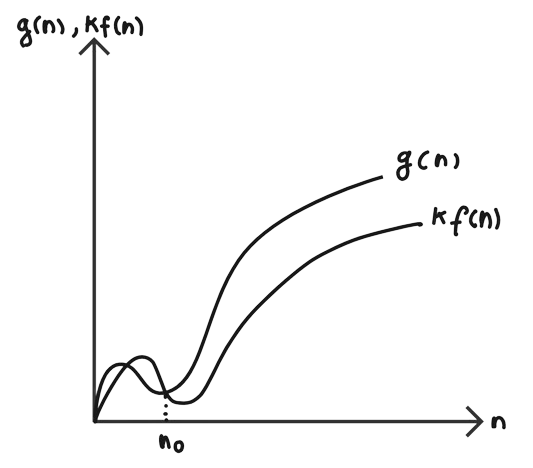
\includegraphics[width=0.4\linewidth]{img/Omega.png}
    \caption{$g(n)\in\Omega(f(n))$.}
    \label{Omega}
\end{figure}

\textbf{Exemplo}

Seja $f(n)=2n^2$, verifique se $f(n)\in\Omega(n^2)$, $f(n)\in\Omega(n\log(n))$ e $f(n)\in\Omega(n)$, utilizando a definição de taxa de crescimento.

Como $n \prec n\log(n) \prec n^2 \approx 2n^2$, então é possível dizer que $2n^2\in\Omega(n^2)$, $2n^2\in\Omega(n\log(n))$ e $2n^2\in\Omega(n)$.

{\raggedleft $\bigtriangleup$ \par}

\subsubsection{Notação $\Theta$}
\

$g(n)\in\Theta(f(n))$($g$ de $n$ está em theta de $f$ de $n$) significa que $f(n)$ é o \textbf{limite assintótico restrito} de $g(n)$, existem constantes $k_0$ e $k_1$ de forma que $0\leq k_0f(n) \leq g(n) \leq k_1f(n), \ \forall n\geq n_0$. Ou seja, o conjunto de funções

\[\Theta(f(n))=\{g: \mathbb{N}_0 \rightarrow \mathbb{R}^{+}: \ \exists k_0, \ k_1, \ n_0 > 0; \ 0\leq k_0f(n) \leq g(n) \leq k_1f(n), \ \forall n \geq n_0 \}.\]

Se $g(n)\in\Theta(f(n))$, então $g(n)\in O(f(n))$ e $f(n)\in\Omega(g(n))$, a recíproca também é válida.

Além disso $g(n)\in\Theta(f(n)) \Leftrightarrow f(n)\in\Theta(g(n))$.

\begin{figure}
  \centering
  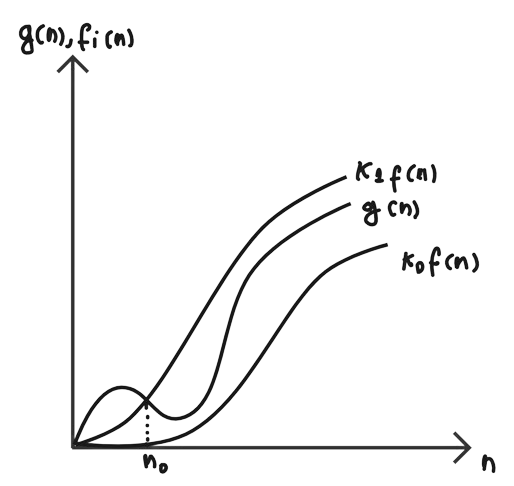
\includegraphics[width=0.4\linewidth]{img/Theta.png}
    \caption{$g(n)\in\Theta(f(n))$.}
    \label{Theta}
\end{figure}

\textbf{Exemplo}

Mostre que $\frac{n^2}{2}-3n \in \Theta(n^2)$.

O problema consiste em encontrar $k_0, \ k_1, \ n_0 > 0$ tais que $k_0n^2\leq \frac{n^2}{2}-3n\leq k_1n^2 \ \forall n\geq n_0$.

Dividindo a expressão por $n^2$

\[k_0\leq \frac{1}{2} - \frac{3}{n} \leq k_1 \ \forall n\geq n_0.\]

Para a inequação da direita $\frac{1}{2}-\frac{3}{n}\leq k_1$, escolhendo $n_0=1$ e $k_1=\frac{1}{2}$ encontra-se $\frac{1}{2} -3 \leq \frac{1}{2}$, satisfazendo a primeira desigualdade.

Na segunda inequação $\frac{1}{2}-\frac{3}{n}\geq k_0$, se escolhermos $k_0=\frac{1}{14} < k_1$ e $n_0=7$ a desigualdade é satisfeita.

Dessa forma, para $n\leq 7$ ou seja$n_0=7$, são escolhidas $k_0=\frac{1}{14}$ e $k_1=\frac{1}{2}$, e pela definição $\frac{n^2}{2}-3n\in\Theta(n^2)$.

{\raggedleft $\bigtriangleup$ \par}

\subsubsection{Notação $o$ e $\omega$}
\

As duas últimas notações são usadas para \textbf{limites assintoticamente não justos}, $o$ para superiores e $\omega$ para inferiores.

Por exemplo, seja $\lambda$ uma constante maior que zero, $\lambda n^2 = O(n^2)$ mas $\lambda n^2 \neq o(n^2)$. Ademais, $\lambda n = o(n^2)$.

\[o(f(n)) = \{g: \mathbb{N}_0 \rightarrow \mathbb{R}^{+}: \ \exists k, n_0 > 0 ; \ 0\leq g(n) < kf(n), \ \forall n \geq n_0\}.\]

Os limites abaixo revelam que à medida que $n \rightarrow \infty$, $g(n)$ torna-se insignificante em relação à $f(n)$.

\[lim_{n\rightarrow\infty} \frac{f(n)}{g(n)}=\infty; \ \ lim_{n\rightarrow\infty} \frac{g(n)}{f(n)}=0.\]

De forma análoga, $\lambda n^2 = \omega(n)$ mas $\lambda n^2 \neq \omega(n^2)$, contudo $\lambda n^2 = \Omega(n^2)$.

\[\omega(f(n)) = \{g: \mathbb{N}_0 \rightarrow \mathbb{R}^{+}:  \ \exists k, n_0 > 0 ; \ 0\leq kf(n) < g(n), \ \forall n \geq n_0\} .\]

Os limites abaixo revelam que à medida que $n \rightarrow \infty$, $f(n)$ torna-se insignificante em relação à $g(n)$.

\[lim_{n\rightarrow\infty} \frac{g(n)}{f(n)}=\infty; \ \ lim_{n\rightarrow\infty} \frac{f(n)}{g(n)}=0.\]

É claro que as notações $o$ e $\omega$ respeitam a identidade de simetria de transposição entre si.

\begin{figure}
  \centering
  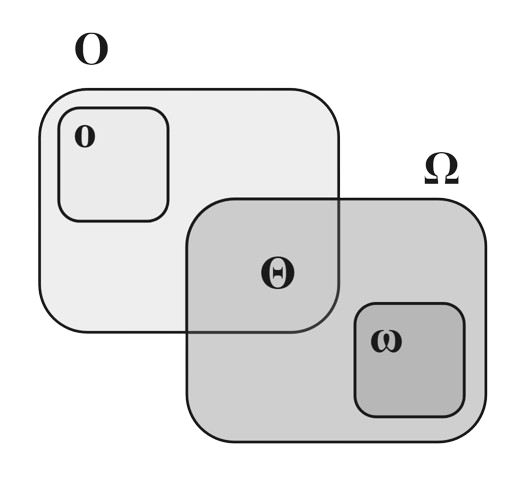
\includegraphics[width=0.4\linewidth]{img/conjuntonotacoes.png}
    \caption{Conjunto de funções nas notações.}
    \label{conjuntonotacoes}
\end{figure}

\textbf{Exemplo}

Prove que $2n\in o(n^2)$ mas $2n^2\notin o(n^2)$.

\[\lim_{n\rightarrow\infty}\frac{2n}{n^2}=0; \ \ \lim_{n\rightarrow\infty}\frac{2n^2}{n^2}=2.\]

Assim, $2n\in o(n^2)$ é uma expressão válida para todos os valores de $k>0$ e $n_0=1$ e como o limite no segundo caso não tende a zero, não existem valores $k>0$ e $n_0$ que satisfaçam a definição da notação $o$, portanto $2n^2\notin o(n^2)$.

{\raggedleft $\bigtriangleup$ \par}

\subsection{Identidades de notação assintótica}
\

As comparações assintóticas respeitam algumas identidades, considerando funções $f$ e $g$ assintoticamente positivas.

\textbf{Reflexividade}
\[f(n)\in\Theta(f(n)).\]

Aplica-se também as notações $O$ e $\Omega$.

\textbf{Transitividade}
\[f(n)\in\Theta(f(n)), \ g(n)\in\Theta(h(n)) \Rightarrow f(n)\in\Theta(h(n)).\]

Aplica-se para todas as outras notações.

\textbf{Simetria}

\[f(n)\in\Theta(g(n)) \Leftrightarrow g(n)\in\Theta(f(n)).\]

\textbf{Outras}

\[O(n+m)=O(n)=O(m).\]
\[O(kn)=kO(n)=O(n).\]

Quando a notação assintótica é utilizada sozinha no lado direito de uma equação como em $n=O(n)$, o sinal de $=$ não representa igualdade e sim que a função $f(n)=n\in O(n)$, sendo unidirecional, assim nunca se deve escrever coisas do tipo $O(n)=n$.

Em equações como a apresentada abaixo $=$ representa igualdade.

\[n^2+n+10=n^2+\Theta(n).\]

Na equação supracitada, a notação assintótica pode ser interpretada como uma função que não é importante definir precisamente.

\[n^2+n+10=n^2+f(n).\]

A função $f(n)$ pertence ao conjunto $\Theta(n)$. Nesse caso, $f(n)=n+10$ que de fato pertence a $\Theta(n)$.

\subsection{O básico das regras de cálculo de complexidade}
\

Como mencionado, a partir de uma inspeção do algoritmo, antes de sua implementação é possível estimar sua complexidade e colocá-la em termos de $O(f(n))$. Algumas estruturas no algoritmo podem ter suas complexidades estimadas rapidamente, outros algoritmos requerem técnicas mais avançadas. O cálculo do número de operações é um problema de contagem, abaixo alguns exemplos simples utilizando os princípios fundamentais da contagem.

Deve-se sempre procurar expressar o custo assintótico de algoritmos da forma mais precisa possível. No caso da notação $O$, essa precisão envolve (1) expressar o limite superior firme do custo assintótico do algoritmo e (2) indicar o caso do algoritmo para o qual esse custo se aplica.

\textbf{Exemplo}

O algoritmo para encontrar um elemento $k$ em um vetor não ordenado de tamanho $n$ tem custo $O(n)$ no pior caso. É possível dizer que no pior caso o algoritmo é $O(n^2)$, no entanto, esse custo não define um limite superior firme, que é $O(n)$ e a função $f(n)=n$ que deve ser usada.

{\raggedleft $\bigtriangleup$ \par}

\subsubsection{Constantes}
\

\textbf{Exemplo}

Operações aritméticas e atribuições levam um custo constante e distinto para serem realizadas. Por exemplo no pseudocódigo abaixo, cada linha tem um custo constante $k_0$, $k_1$ e $k_2$ respectivamente. Frequentemente, consideramos todas com custo $1$, mas na realidade isso é falso, elas possuem custos distintos.

\begin{lstlisting}[language=C, frame=single]
    int a:= 2
    int b:= 7
    int a:=a+b
\end{lstlisting}

A chamada \textbf{função de complexidade}, são os valores explícitos $f(n)=k_0+k_1+k_2=k_3$ ou $f(n)=3$, a \textbf{ordem de complexidade} é a ordem expressa em notação assintótica apenas com os termos dominantes, ignorando constantes e termos assintoticamente irrelevantes, $f(n)=O(1)$.

{\raggedleft $\bigtriangleup$ \par}

\subsubsection{Laços de iteração}
\

\textbf{Exemplo 1}

O algoritmo representado por pseudocódigo abaixo está somando elementos de um vetor $V$ utilizando um laço de iteração \textit{for}.
\begin{lstlisting}[language=C, frame=single]
    int soma(V,n) 
    {
        int s:= 0
        for(i:=0; i<n; i++)
            s:=s+V[i]

        return s
    }
\end{lstlisting}

Primeiramente vamos estimar a complexidade do tempo de execução do algoritmo. 

(1) Atribuir o valor 0 para $s$ tem custo 1; 

(2) No laço de iteração \textit{for} $i:=0$ tem custo 1, $i++$ é feito $n$ vezes e a comparação $i<n$, $n+1$ vezes, é possível então dizer que o \textit{for} tem custo $2n+2$, no entanto  o importante é a operação mais realizada, a de \textit{comparação} $i<n$, com custo $n+1$;

(3) A \textit{atribuição} $s:=s+V[i]$, dentro do laço de repetição é no total realizada $n$ vezes, portanto tem custo $n$.

Somando as complexidades em (1), (2) e (3) obtemos $g(n)=2n+3$. E podemos dizer $g(n)=O(n)$.

A complexidade de espaço nesse algoritmo também pode ser estimada.

(1) As variáveis $n$, $s$ e $i$ tem custo 1, somando temos 3;

(2) $V$ é um vetor que armazena $n$ variáveis e tem custo $n$;

Somando as complexidades de (1) e (2), obtemos $S(n)=n+3$ e $S(n)=O(n)$.

{\raggedleft $\bigtriangleup$ \par}

\textbf{Exemplo 2 (Laços aninhados)}

Um caso extremamente comum são os \textbf{laços de iteração aninhados}.
\begin{lstlisting}[language=C, frame=single]
    for(i:=0; i<n; i++)
        for(j:=0; j<n; j++)
            //procedimento
\end{lstlisting}

Note que a cada iteração do primeiro laço, o segundo executa $n+1$ comparações, mas como o primeiro laço repete $n$ iterações, obtemos $g(n)=n(n+1)=n^2+n$ e $g(n)=O(n^2)$.

Generalizando, sejam $i_0, \ i_1, ... \ , i_{k-1}$, $k$ variáveis distribuídas entre $k$ laços de iteração, onde $i_k<n$ e $i_k++$ para todo laço de iteração, ignorando outros procedimentos, podemos estimar a complexidade como $g(n)=O(n^k)$.

{\raggedleft $\bigtriangleup$ \par}

\textbf{Exemplo 3}

Nos laços de iteração aninhados abaixo, repare a comparação $j<i$.

\begin{lstlisting}[language=C, frame=single]
    for(i:=0; i<n; i++)
        for(j:=0; j<i; j++)
        //procedimento
\end{lstlisting}

(1) O primeiro laço com o iterador $i$ realiza $n+1$ comparações;

(2) No segundo laço $j$ varia de $0$ a $k$ a cada vez que $i:=k$, sendo $0\leq k\leq n$. Dessa forma, o procedimento é executado $0+1+2+3+...+n = \frac{n(n+1)}{2}$ vezes.

Sendo assim, a complexidade do algoritmo é $O(n^2)$.

{\raggedleft $\bigtriangleup$ \par}

\textbf{Exemplo 4 (Passos diferentes)}

Repare no passo do laço de repetição abaixo $i:=i+k$. Onde $k$ é alguma constante

\begin{lstlisting}[language=C, frame=single]
    for(i:=0; i<n; i:=i+k)
        //procedimento
\end{lstlisting}

Se $i$ é incrementado de $k$ em $k$, o procedimento é executado $\frac{n}{k}$ vezes e o laço realiza $\frac{n}{k}+1$ comparações. A complexidade do algoritmo é $O(n)$.

{\raggedleft $\bigtriangleup$ \par}

\textbf{Exemplo 5 (Condição de parada)}

Há casos em que o laço de iteração não é tão evidente, podendo ser o caso de inspecionar a condição de parada, ou seja, a condição que deve ser satisfeita para o laço de iteração parar de executar as operações dentro dele. No exemplo abaixo a condição de parada é $j > n$.

\begin{lstlisting}[language=C, frame=single]
    int j:= 0
    for(i:=0; j <= n; i++)
        j:=j+i
\end{lstlisting}
Primeiramente, qual o comportamento da variável $j$ a medida que $i$ é incrementada ?

(1) O comportamento de $j$ é descrito na tabela abaixo;

\newpage
 
\begin{table}
  \centering
  \begin{tabular}{cc}
    \textbf{i} & \textbf{j} \\
    \hline
    $0$ &  $0$ \\
    $1$ &  $0+1 = 1$ \\
    $2$ & $0+1+2 = 3$ \\
    $k$ &  $0+1+...+k = \frac{k(k+1)}{2}$ \\
  \end{tabular}
\end{table}

(2) Vamos assumir que a condição de parada foi alcançada, ou seja $j>n$. Isso significa que para algum valor $i=k$, $j>n$ e como $j = \frac{k(k+1)}{2} > n$;

(3)
\[\frac{k(k+1)}{2} =  \frac{k^2+k}{2}> n \Rightarrow k^2+k > 2n \Rightarrow k^2 > n \Rightarrow k > \sqrt{n}. \]

A complexidade desse algoritmo é $O(\sqrt{n})$.

{\raggedleft $\bigtriangleup$ \par}

\textbf{Exemplo 6}

\begin{lstlisting}[language=C, frame=single]
    for(i:=0; i<n; i:=i*2)
        //procedimento
\end{lstlisting}

(1) A variável $i$ cresce em potências de base $2$ e assume um valor $2^k$;

(2) Assumindo que a condição de parada $i\geq n$ foi atingida, então $2^k \geq n$ e quando $2^k = n$, obtemos $k = \log_2(n)$;

(3) O procedimento é executado $\lceil \log_2(n) \rceil$ vezes.

A complexidade do algoritmo é $O(log(n))$.

{\raggedleft $\bigtriangleup$ \par}

\textbf{Exemplo 7}

\begin{lstlisting}[language=C, frame=single]
    for(i:=0; i*i<n; i++)
        //procedimento
\end{lstlisting}

A condição de parada do laço de iteração é $i^2  \leq n$, o algoritmo tem complexidade $O(\sqrt{n})$.

{\raggedleft $\bigtriangleup$ \par}

\subsubsection{Fases}

Se um algoritmo possui diversas fases, a complexidade do tempo de execução será a da fase com maior complexidade.

\textbf{Exemplo 1}

No pseudocódigo abaixo, o laço com maior complexidade é o segundo, $O(n^2)$. A complexidade do algoritmo é $O(n^2)$.

\begin{lstlisting}[language=C, frame=single]
    for(i:= 0; i<n; i++)
        // procedimento
    
    for(i:= 0; i<n; i++)
        for(j = 0; j<n; j++)
            //procedimento
\end{lstlisting}
    
{\raggedleft $\bigtriangleup$ \par}

\textbf{Exemplo 2 (Dependência de fases)}  

No pseudocódigo abaixo, a variável $p$ cria uma dependência entre os laços, e embora eles não estejam aninhados, a complexidade do procedimento executado no segundo laço depende da complexidade do primeiro.

\begin{lstlisting}[language=C, frame=single]
    int p:= 0
    for(i:= 0; i<n; i=i*2)
        p++
    
    for(i:= 0; i<p; i=i*2)
        //procedimento
\end{lstlisting}

(1) A variável $p$ é incrementada $\lceil \log_2(n) \rceil$ vezes no primeiro laço de iteração;

(2) O procedimento do segundo laço de repetição é executado $\log_2(p) = \log_2(\log_2(n))$ vezes.

A complexidade nessa caso é $O(\log\log(n))$.

{\raggedleft $\bigtriangleup$ \par}

\subsubsection{Várias variáveis}
\

Em alguns casos a complexidade pode depender de mais de uma variável e sua ordem de magnitude estará em função dessas variáveis.

\textbf{Exemplo}  

\begin{lstlisting}[language=C, frame=single]
    for(i:= 0; i<n; i++)
        for(j:= 0; m; j++)
            //procedimento
\end{lstlisting}

Nesse caso a complexidade é $O(nm)$.

{\raggedleft $\bigtriangleup$ \par}

\subsubsection{Recursão}
\

A complexidade do tempo de execução de funções recursivas depende do número de chamadas e da complexidade de cada chamada.

\textbf{Exemplo 1} 

\begin{lstlisting}[language=C, frame=single]
    fatorial(n)
    {
        if(n=0)
            return 1

        n*fatorial(n-1)
    }
\end{lstlisting}

(1) Cada chamada faz uma comparação e tem complexidade $O(1)$ (constante);

(2) Dada uma entrada $n$ a função faz $n-1$ chamadas recursivas;

A complexidade total é o produto da complexidade de cada chamada e da complexidade da quantidade de chamadas, dessa forma a complexidade é $O(n)$.


{\raggedleft $\bigtriangleup$ \par}

\textbf{Exemplo 2} 

\begin{lstlisting}[language=C, frame=single]
    void funcao(n)
    {
        if(n=1)
           return

        funcao(n-1)
        funcao(n-1)
    }
\end{lstlisting}

(1) Cada função gera duas chamadas do mesmo tipo, as próximas duas fazem juntas quatro chamadas, as próximas quatro, oito e assim por diante;

(2) quando as chamadas chegam em $funcao(1)$ foram feitas $2^{n-1}$ chamadas.

A complexidade é $O(2^n)$.
 

{\raggedleft $\bigtriangleup$ \par}

\subsection{Classes de complexidade}

Na análise de algoritmos existem classes de complexidade muito comuns. Do ponto de vista assintótico a seguinte hierarquia de funções pode ser definida

\[1\prec \log(\log(n)) \prec log(n) \prec \sqrt[k]{n} \prec n \prec n\log(n) \prec n^k \prec n^{\log(n)} \prec k^n \prec n!\prec n^n.\]

Onde $k$ é uma constante maior que zero.

A hierarquia de funções supracitadas indica que as funções mais a direita tem uma \textbf{ordem de crescimento} ou \textbf{ordem de magnitude} maior. Ou seja, quando $n\rightarrow\infty$, assumem valores mais significativos.

\begin{figure}
  \centering
  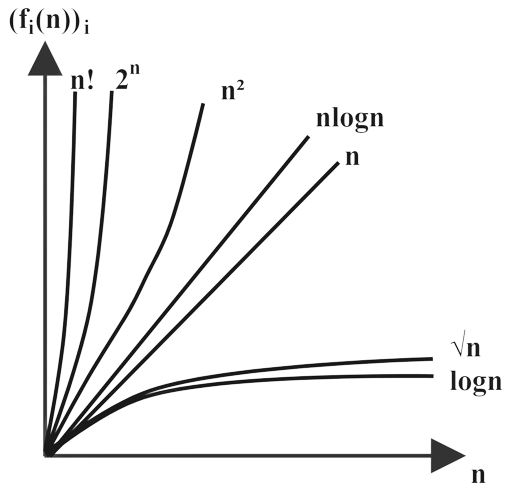
\includegraphics[width=0.4\linewidth]{img/Classes.png}
    \caption{Esboço, algumas funções da hierarquia.}
    \label{Hierarquia}
\end{figure}

\subsubsection{Lista de classes de complexidade}
\

$O(1)$ Dizemos que a complexidade do tempo de execução é \textbf{constante}, geralmente quando é utilizada uma formula fechada, não dependendo do tamanho da entrada;

$O(log(n))$ A complexidade é dita \textbf{logarítmica}, geralmente o tamanho da entrada é dividido por um fator, um exemplo de algoritmo é a \textbf{busca binária};

$O(\sqrt{n})$ É uma complexidade de \textbf{raiz quadrada} que fica aproximadamente no meio da entrada já que $\sqrt{n} = \frac{\sqrt{n}}{n}$;

$O(n)$ Executa em tempo \textbf{linear}, geralmente é o melhor caso de complexidade possível de alcançar, já que muitas vezes é preciso acessar n posições pelo menos uma vez;

$O(nlog(n))$ A complexidade \textbf{nlog(n)} é um forte indício de que a entrada está sendo ordenada ou que há uma \textbf{estrutura de dados} com operações de complexidade em tempo de execução de $O(log(n))$;

$O(n^2)$ Um algoritmo com complexidade de tempo de execução \textbf{quadrática} geralmente aparece em laços de iteração aninhados; 

$O(n^3)$ É dito um algoritmo \textbf{cúbico};

$O(2^n)$ Em geral os casos $k^n$ são chamados \textbf{exponenciais}, no entanto $2^n$ é um caso particular, pois é o número de subconjuntos de um conjunto discreto finito, o que pode revelar que o algoritmo itera por todos os subconjuntos da entrada;

$O(n!)$ Uma complexidade \textbf{fatorial} geralmente indica que o algoritmo itera por todas as permutações da entrada.

\subsection{Pior caso, melhor caso e caso médio}
\

Um mesmo algoritmo pode desempenhar diferentes complexidades dependendo da entrada. O melhor caso de uma busca em um vetor por exemplo, ocorre quando o primeiro elemento é o elemento procurado, e o pior caso quando o elemento não se encontra no vetor.

O algoritmo de ordenação \textit{quicksort} por exemplo, apresenta seu caso médio com complexidade $O(n\log(n))$ e seu pior caso com complexidade $O(n^2)$.

O cálculo de complexidade do caso médio é bem mais complicado, Ele requer a probabilidade $P$ da ocorrência de uma entrada.

Felizmente, na maioria da vezes, estamos interessados no pior caso de complexidade do algoritmo.